% arara: xelatex: {shell: true}
% arara: biber
% arara: xelatex: {shell: true}
% arara: xelatex: {shell: true}
% arara: xelatex: {shell: true}
\documentclass[letterpaper,10pt]{article}
\usepackage[margin=1in]{geometry}
\usepackage{newfloat}
\usepackage{hyperref}
\usepackage{graphicx}
\usepackage[font=small,labelfont=bf]{caption}
%\usepackage{draftwatermark}
\usepackage{fancyhdr}
\usepackage{makecell}
\usepackage{wrapfig}
\usepackage{parskip}
\usepackage[section]{placeins}
\usepackage{epigraph}
%\usepackage{sourcecodepro}
\usepackage{fontspec}
\usepackage[toc,nonumberlist,xindy]{glossaries}
\usepackage{xelatexemoji}
\usepackage{relsize}
%\setmonofont[Scale=0.7]{Source Code Pro}
\setmonofont[Scale=0.8]{Unifont}
\defaultfontfeatures{Ligatures=TeX}
\usepackage[table]{xcolor}
%\usepackage{pdfpages}
\usepackage[titletoc,title]{appendix}
\usepackage{tipa}
\newfontfamily\greekfont{Noto Sans}
\definecolor{dsscawpurp}{HTML}{b079b0}
\definecolor{dsscawpurpcap}{HTML}{6c286c}
\usepackage[font={color=dsscawpurpcap},labelfont={sc}]{caption}
\usepackage[backend=biber,
date=iso,
seconds=true,
style=numeric,
bibencoding=utf8,
]{biblatex}

\tracinglostchars=2

%\SetWatermarkText{DRAFT}
%\SetWatermarkScale{1}

\hypersetup{
  colorlinks=true,
  linkcolor=blue,
  pdftitle={Proposal for Prefix ZW Operators},
}

\addbibresource{\jobname.bib}
\newenvironment{denseitemize}{
  \begin{itemize}
      \setlength{\itemsep}{0pt}
}{
  \end{itemize}
}

\pagestyle{fancy}
\rhead{
  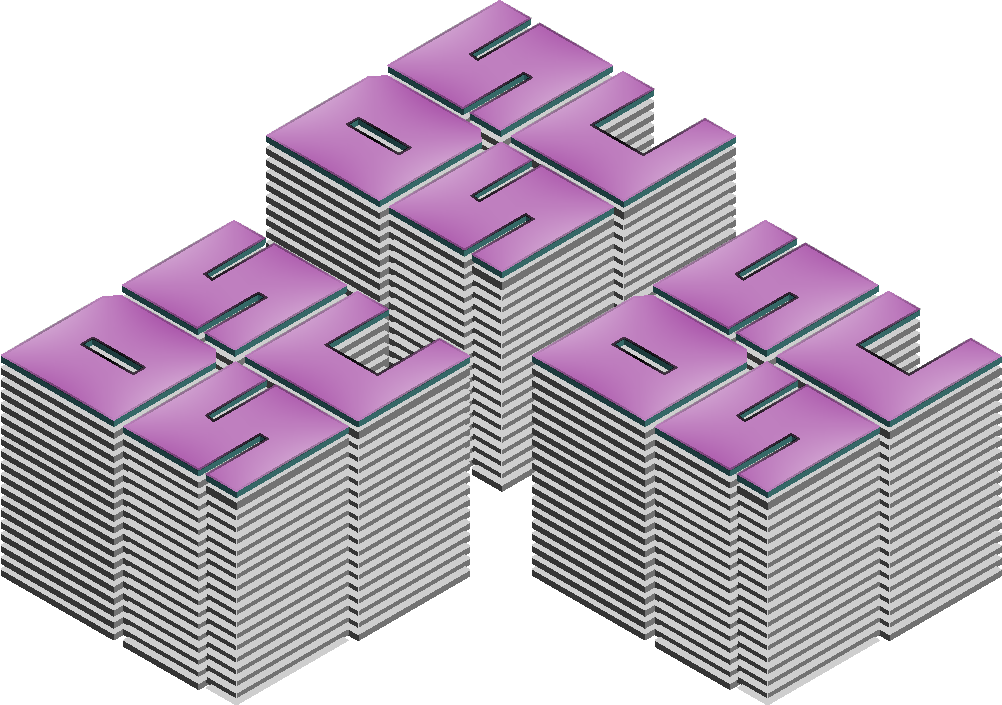
\includegraphics[height=\fontcharht\font`\D,keepaspectratio=true]{../dsscaw-hdr.pdf}
  \textcolor{dsscawpurp}{DSSCAW Technical Report \#005}
}

\title{Proposal for Prefix ZW Operators}
\author{nick black, consulting scientist\\
\texttt{nickblack@linux.com}
}

%%%%%%%%%%%%%%%%%%%%%%%%%%%%%%%%%%%%%%%%%%%%%%%%%%%%%%%%%%%%%%%%%%%%%%%%
\begin{document}
%%%%%%%%%%%%%%%%%%%%%%%%%%%%%%%%%%%%%%%%%%%%%%%%%%%%%%%%%%%%%%%%%%%%%%%%
%
\includepdf{media/frontcover.pdf}
%\date{March 24, 2020}
\maketitle
\date{}
\vspace{1in}
\begin{abstract}
When processing a stream of Unicode, there are several cases where it
is useful or even necessary to know that a codepoint is only part of a
ZWJ sequence. This is not possible with existing ZWJ semantics, since
the ZWJ arrives only after each non-terminating combined character. I
propose stacking, prefixing ZWJ and ZWNJ, indicating that the subsequent two
encoded codepoints and/or ZWJ sequences are to be combined into a single
ZWJ sequence. Backwards compatibility is maintained.
\end{abstract}
\thispagestyle{empty}
%%%%%%%%%%%%%%%%%%%%%%%%%%%%%%%%%%%%%%%%%%%%%%%%%%%%%%%%%%%%%%%%%%%%%%%%

\section{Introduction}
As the author of a modern library for TUIs and character graphics\cite{notcurses},
I've spent significant time over the past two years working with
complex Unicode in interactive environments. Interactivity, and more
fundamentally streaming, adds complexity to handling Unicode, especially
with regard to combining characters, ZWJ sequences\cite{zwjseqs}, and
segmentation\cite{segmentation}. The entirety of an EGC or ZWJ sequence
might not be available when the non-terminating character(s) are read;
in the interactive or simply highly latent case, subsequent elements of
the sequence might not be available even after user-perceivable delay.
It is even possible that subsequent elements are never received. What is
a program to do with the base characters in the interim?

The widespread UTF-8 encoding\cite{RFC3629} allows an encoded character's
length to be determined from its first byte. Assuming a byte-oriented
transport, there is thus never any question as to whether the entire encoded
character has been received. The (non-trivial) prefix of a given encoded
character cannot be the prefix of any other result of valid UTF-8 encoding.
EGCs and ZWJ sequences do not enjoy this happy property; many (but not all)
prefixes of these text elements are themselves valid standalone EGCs.

\section{The Valid Prefix Problems}

The most fundamental problem due to valid prefixes is that \textbf{something
sensible can be done with the prefix in isolation}. This is not possible when
reading UTF-8; if we receive an incomplete encoded character, this fact is
obvious. If we receive a message ending in such an incomplete character, we
know that it was truncated; the user can be informed of the truncation, and
certainly no incorrect glyph will be substituted. There need be no feedback
to a typing user, as nothing they might type would generate such an incomplete
output.

This is not true for EGCs or ZWJ sequences. Most catastrophically, a
truncation can change the entire meaning of a sequence, replacing it with
a different (but semantically viable) concept. For instance, imagine
a passenger liner has received the message "Heads up! Your path will
pass by 🏴". It is not unreasonable to assume that the passengers will
be instructed to bring out their cameras, in the hope of seeing the
New Zealand All-Blacks and one of their mighty \textit{haka} dances.
In truth, of course, they ought have drawn their ⚔️s; the missing U+200D
and U+2620 would have indicated the presence of pirates \xelatexemoji{1f3f4-200d-2620-fe0f}.
Were I to describe the action of \textit{Indiana Jones and the Temple of Doom}
as "In the hand of Mola Ram is held the victim's \xelatexemoji{2764}", that's a completely
different subtext than "\xelatexemoji{2764-fe0f-200d-1f525}". A manager
delegating a task to her Sudanese mermaid subordinate might address Aarifa
as \xelatexemoji{1F9DC-1F3FE-200D-2640-FE0F} (``mermaid: medium-dark skin
tone''); should that be truncated to \xelatexemoji{1f9dc} (``merperson''),
she's not only created a non-inclusive environment for BIPOC merpeople,
but inadvertently misgendered Aarifa, now a crime in several jurisdictions
(not to mention possibly confusing any non-binary merployees). This is
no way to solve tech's diversity problem.

There are further issues. In an interactive environment, typing a ZWJ
sequence usually involves entering a series of characters. What is to be
displayed following the first valid prefix? If the valid prefix happened
to be wider than the resulting sequence\footnote{I do not believe this to
be possible through Unicode 13.1.}, it could lead to a false line
wrap. A glyph similar to (but distinct from) the sequence glyph might be
confusing, and catalyze errors. Alternatively, an editor might wish to
indicate that further input is desired; this is not possible with infix
ZWJ. Several threads might pull encoded characters from a common buffer;
while a thread can be certain it is atomically pulling a complete UTF-8
character, it cannot be certain that it has pulled the entirety of an
EGC or ZWJ sequence. The choice is then either to wait an arbitrary amount
of time for further possible characters whenever a valid prefix is
received (not allowing earlier characters to be processed), or for some
other thread to retrieve the suffix, and likely throw an error.

\section{Resolution via Prefix ZWJ}

For EGCs made up of combining characters, there is no general way to
solve this problem, but for ZWJs with their explicit binding control,
a solution is at hand: introduce the bound sequence with a \textit{prefix}
ZWJ, henceforth known as PZWJ. Like the infix ZWJ, PZWJ always works on two
text elements. Like the infix ZWJ, PZWJ can be chained to use several
component characters. Unlike the infix ZWJ, PZWJ completely and
unambiguously describes the resulting structure \textit{from the beginning of
the structure}. Concatenation is associative\cite{automata}, and thus all
possible distributions of $N-1$ PZWJs across $N$ characters yield the same
result.

\section{Details of PZWJ}

PZWJ and PZWNJ will live in the Supplemental Punctuation block, occupying the
unused codepoints \texttt{U+2E5C} and \texttt{U+2E5D}, with the names
\texttt{Prefix Zero Width Joiner} and \texttt{Prefix Zero Width Non-Joiner}.
The least significant hex digits have been chosen to match ZWJ/ZWNJ.

PZWJ binds more tightly than infix ZWJ. If PZWJ binds less tightly than ZWJ,
it defeats the entire point. Right-associativity, as much as it applies at
all, follows directly from prefix notation. It is expected that text making
use of PZWJ will forego ZWJ entirely, but a PZWJ sequence may form the right-hand
side of a ZWJ sequence. It \textbf{must not} form the left-hand side of a
ZWJ sequence (this would defeat the point), though it can form the right-hand
side. A PZWJ sequence can form one or both sides of another PZWJ sequence.
Canonicalization will continue to admit ZWJ sequences, but any PZWJ sequence
\textbf{must} canonicalize as PZWJs only, built up entirely using the form

\begin{center}
\texttt{PZWJ \{base character\} \{PZWJ sequence or base character\}}
\end{center}

This allows canonicalizing mixed ZWJ and PZWJ intro pure PZWJ in O(1) space,
in a single pass, from either left-to-right or right-to-left. All Unicode ZWJ
sequences can thus be unambiguously and mechanically rewritten as canonical
PZWJ sequences.

PZWJ and PZWNJ have equivalent precedence.

If a stream terminates without providing all necessary elements of a PZWJ
sequence, this can be detected. The mutilated PZWJ sequence can be passed
through, since it cannot be interpreted as a valid form. The presence of
such a malformed trailer \textbf{should} be indicated to the user via some
means.

\section{Contact Info}
nick black\\
Dirty South Supercomputers and Waffles, LLC\\
855 Peachtree St. NE\\
Suite 3204\\
Atlanta, GA 30308

\pagenumbering{roman}

%%%%%%%%%%%%%%%%%%%%%%%%%%%%%%%%%%%%%%%%%%%%%%%%%%%%%%%%%%%%%%%%%%%%%%%%
\addcontentsline{toc}{section}{References}
\printbibliography
\phantomsection
\cleardoublepage
\end{document}
